\documentclass[a4paper, 11pt]{article}
\usepackage[utf8]{inputenc}

%Margins 
\usepackage[a4paper, left=1.27cm,top=1.27cm,right =1.27cm, bottom = 1.4cm]{geometry}

%Load packages
%Algemene packages
\usepackage{babel}
\usepackage{slantsc}
\usepackage{array}
\renewcommand{\arraystretch}{2}
\usepackage{multicol}
\usepackage{multirow}
\usepackage{amsmath}
\usepackage{amsfonts}
\usepackage{booktabs}

%Opsommingen
\usepackage{enumerate}


%Afbeeldingen
\usepackage{graphicx}
\usepackage{wrapfig}

%Gekleurde tekstboxen 
\usepackage[most]{tcolorbox}

%Stop indent
\setlength{\parindent}{0pt}

%Font
\usepackage{cmbright}
\usepackage[OT1]{fontenc}

%Headers and footers
\usepackage{fancyhdr}

\pagestyle{fancy}
\fancyhf{}
\renewcommand{\headrulewidth}{0pt}
\renewcommand{\footrulewidth}{0pt}
\fancyhead[LE,RO]{}
\fancyhead[RE,LO]{}

%Logo in footer
\usepackage{lastpage}
\lfoot{}
\cfoot{\vspace{-5mm} \thepage}
\rfoot{}

%Voorbeeldtekst
\usepackage{lipsum}

%Meerdere kolommen
\usepackage{multicol}
\setlength{\columnsep}{1cm}

%Whitespace na section
\usepackage[compact]{titlesec}  
\titlespacing{\section}{0pt}{2pt}{0pt}

%Tekst kleur
\usepackage{xcolor}

%Nieuwe kleur
%\definecolor{ugent_blue}{rgb}{0.04706, 0.13725, 0.26667}
\definecolor{ugent_blue}{RGB}{30, 100, 200}

%Nummering sections
\renewcommand\thesection{\arabic{section}}
\renewcommand\thesubsection{\thesection.\arabic{subsection}}

%Lay-out hoofdingen
\titleformat*{\section}{\bfseries \normalfont}
\usepackage{sectsty}
\sectionfont{\color{ugent_blue}}
\titlespacing\section{0pt}{10pt plus 4pt minus 4pt}{0pt plus 2pt minus 2pt}

\raggedbottom


%other shit that may be useful
\usepackage{multicol,caption}
\usepackage{mathtools}
\raggedbottom
\newcommand{\HRule}{\hrule}
\abovedisplayskip0pt
\renewcommand{\arraystretch}{1.5}
\newcolumntype{M}[1]{>{\centering\arraybackslash}m{#1}}
\usepackage{lscape}
\newenvironment{Figure}
  {\par\medskip\noindent\minipage{\linewidth}}
  {\endminipage\par\medskip}
\usepackage{float}
\usepackage{hyperref}
\newcommand\myfigure[1]{%
\medskip\noindent\begin{minipage}{\columnwidth}
\centering%
#1%
%figure,caption, and label go here
\end{minipage}\medskip}
\usepackage{caption}
\usepackage{subcaption}
\usepackage{tabularx}
\usepackage{enumerate}
\usepackage{enumitem}

\raggedbottom
\raggedcolumns


\usepackage{biblatex} %Imports biblatex package
\addbibresource{sample.bib} %Import the bibliography file

%figures
\graphicspath{{figures/}}


\begin{document}

%Load heading of document
%ugent color
{\color{ugent_blue} \hrule\hrule\hrule}

\vspace*{-0.43mm}
\colorbox{ugent_blue}{\color{white} \bf Report Biomechanics}\\

\noindent\begin{minipage}{0.7\textwidth}% adapt widths of minipages to your needs
{\LARGE \bf \color{ugent_blue} Clinical Movement Analysis Lab Assignment 2022}\\[2mm]

%
{\large Vincent Belpaire}\\
{Supervisor: Prof. Malcolm Forward}\\


{\small University of Ghent}\\
{\small Faculty of Engineering and Architecture}\\
{\small Bachelor of Science: Biomedical Engineering}\\
\end{minipage}%
\hfill%
\begin{minipage}{0.3\textwidth}
\vspace{-2.2cm}
\begin{center}

\includegraphics[width=\linewidth]{ugent_logo}
\end{center}
\end{minipage}\\


\section{Introduction}

The aim of this project is to simulate the behavior of voltages and currents in a lossless transmission line in function of time and space. To accomplish this objective, the Finite-Difference Time-Domain method (FDTD) was used. This method makes use of a leapfrog scheme in both time and space and turns a continuous problem in discrete equations. The transmission line studied in this project is depicted in Figure~\ref{fig:TL} and its discretized version in Figure~\ref{fig:TLD}.

\begin{figure}[h!]
    \centering
    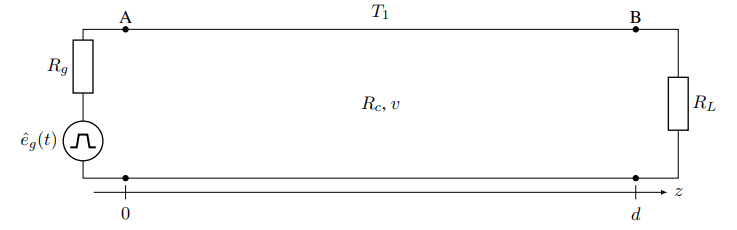
\includegraphics[scale=0.75]{figures/TL.png}
    \caption{Transmission line}
    \label{fig:TL}
\end{figure}

\begin{figure}[h!]
    \centering
    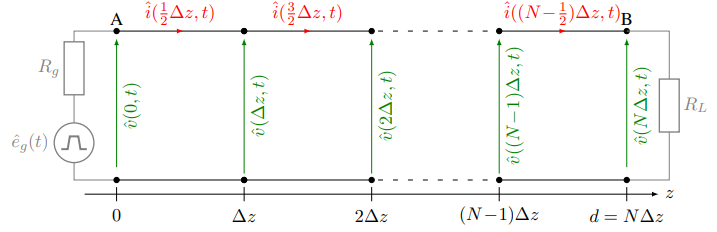
\includegraphics[scale=0.75]{figures/TLD.png}
    \caption{Discretization of the transmission line}
    \label{fig:TLD}
\end{figure}

In the first section, the correct update equations and constants are derived. Using this information, the behavior of a bit traveling through the transmission line is studied, both with default values and with varying parameters. This is all considered with just a resistor as load. Eventually a capacitor is added in parallel to the load. This changes the bit behavior substantially. To conclude the report, an application of transmission line theory inside the field of biomedical engineering is discussed.


%Start writing your repot...

\section{A bit traveling through a lossless transmission line}

    \subsection{Numerical implementation}

In the assignment paper the update functions are given as 
\begin{align}
    \tilde{I}^{m+\frac{1}{2}}_{n+\frac{1}{2}} = \tilde{I}^{m-\frac{1}{2}}_{n+\frac{1}{2}} + \alpha\left(V^{m}_{n} - V^{m}_{n+1}\right) \label{update}, \quad\quad
    V^{m+1}_n = V^{m}_{n} + \alpha\left(\tilde{I}^{m+\frac{1}{2}}_{n-\frac{1}{2}}-\tilde{I}^{m+\frac{1}{2}}_{n+\frac{1}{2}}\right),  
\end{align}
with
\begin{equation}
\alpha \triangleq \frac{v\Delta t}{\Delta z}
    \label{alpha}
\end{equation}

the dimensionless Courant factor and
\begin{equation}
    \tilde{I}^{m+\frac{1}{2}}_{n+\frac{1}{2}} = I^{m+\frac{1}{2}}_{n+\frac{1}{2}}R_c
    \label{Itil}
\end{equation}
the rescaled current.

The boundary condition at the generator ($z=0$) is briefly discussed in the assignement but is not finalized. It's final form at $z=0$ is
\begin{equation}
    V^{m+1}_{0} = K_{1}V^{m}_{0} + 2\kappa_{1}\left(E^{m+\frac{1}{2}}_{g}\frac{R_c}{R_{g}} - \tilde{I}^{m+\frac{1}{2}}_{\frac{1}{2}}\right)
\end{equation}
where
\begin{align}
    K_{1} & = \frac{R_{g}-\alpha R_{c}}{R_{g}+\alpha R_{c}},\\
    \kappa_{1} & = \frac{\alpha R_{c}}{R_{g}+\alpha R_{c}},
\end{align}
are two dimensionless constants which will be discussed in a following section.\\

At the load ($z=d$) a similir situation occurs as at the generator ($z=0$), namely there is a resistance. This is depicted in figure \ref{fig:Rl}.

\begin{figure}[h!]
    \centering
    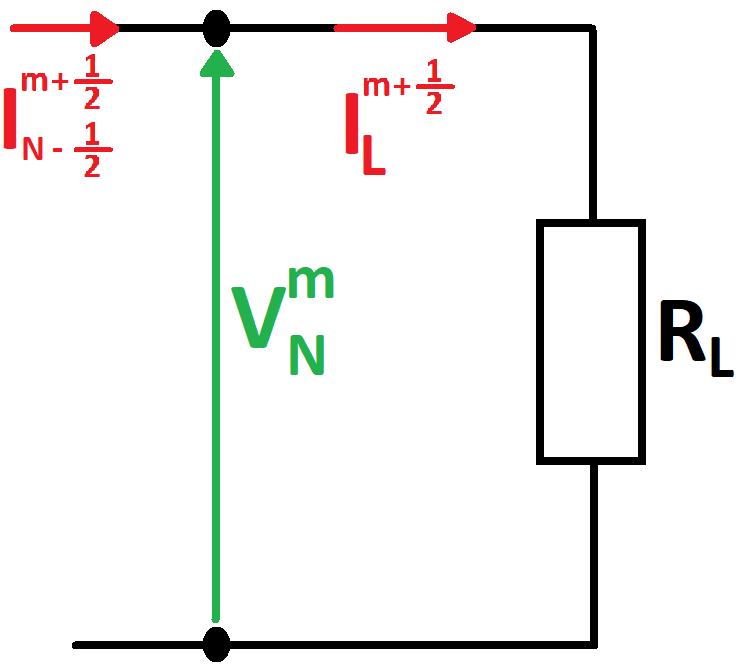
\includegraphics[scale=0.25]{BC2}
    \caption{Boundary situation at the $z=d$}
    \label{fig:Rl}
\end{figure}

The voltage update equation becomes:
\begin{equation}
    V^{m+1}_{N} = V^{m}_{N} + \frac{2\Delta t}{C\Delta z}\left(I^{m+\frac{1}{2}}_{N-\frac{1}{2}} - I^{m+\frac{1}{2}}_{L}\right)
    \label{BC2}
\end{equation}
Kirchoff's voltage law in discretized form states that
\begin{align}
    I^{m+\frac{1}{2}}_{L} & = \frac{V^{m+\frac{1}{2}}_{N}}{R_{L}}\nonumber\\
    & = \frac{V^{m}_{N}+V^{m+1}_{N}}{2R_{L}}
    \label{IL}
\end{align}
Subsituting (\ref{IL}) in (\ref{BC2}) and using the same relations as for $z=0$ yields, 
after some rearrangements:
\begin{equation}
    V^{m+1}_{N} = K_{2}V^{m}_N + 2\kappa_{2}\tilde{I}^{m+\frac{1}{2}}_{N-\frac{1}{2}},
\end{equation}
where
\begin{align}
    K_{2} & = \frac{R_{L}-\alpha R_{c}}{R_{L}+\alpha R_{c}},\\
    \kappa_{2} & = \frac{\alpha R_{c}}{R_{L}+\alpha R_{c}},
\end{align}
are two dimensionless constants which also will be discussed in a following section.

    
%In this section, the numerical analysis of a bit traveling through a lossless transmission line is %established ({\bf Figure CIRCUIT}). To this end, a rough analytical estimation of the simulation is %made

\subsection{General behavior of a bit traveling through a transmission line}\label{gbh}
This section aims to predict, and thus validate, the behavior of the numerical simulation of the voltage in a LTL. A rough analytical approach is used, since it gives more insight in the physical nature of the problem.  \\

Rearranging the telegrapher's equations for a LTL yields

\begin{equation}
\frac{\partial^2\hat{v}(z, t)}{\partial z^2} - k^2\frac{\partial^2 \hat{v}(z, t)}{\partial t^2} = 0, \quad k = \frac{1}{c}= \sqrt{LC} = \mathrm{cte}.
\label{tele}
\end{equation}

This means that $\hat{v}$ satisfies the wave equation and thus can be written as a superposition of two voltage waves traveling in opposite directions with constant speed $c$. That is,

\begin{equation}
\hat{v}(z, t) = \underbrace{\hat{v}^{+}(z - ct)}_{\text{forward wave}} + \underbrace{\hat{v}^{-}(z + ct)}_{\text{backward wave}}.
\end{equation}

Realising that the voltage and current are related;

\begin{equation}
\hat{i}(z, t) = \frac{1}{R_c}(\hat{v}^{+}(z, t) - \hat{v}^{-}(z, t)),
\end{equation}

with $R_c = \sqrt{\frac{L_{TL}}{C_{TL}}}$ and $L_{TL}$, $C_{TL}$ p.u.l. inductance resp. capacitance of the TL, a constant that depends on the characteristics of the TL, hence the name characteristic impedance. Although it has the units of resistance ($\Omega$) it is not reactive; there is no energy dissipation over the TL. The characteristic impedance can be interpreted as a scale for (1) the current to voltage amplitude when there is only a forward or backward wave present in the TL and (2) the dissipation of energy to the load or generator (\ref{ref1}). Furthermore, the CI is the consequence of the model we provided for the TL; it counts for the p.u.l capacitance and inductance (depend on type of TL). In further sections, $R_c$ is assumed to be finite and constant.


    \subsection{Effect of varying $\tau_h$ and $\tau_r$}
The bit that is sent through the transmission line model is defined by the rising time ($\tau_r$) and a bit time ($T_{bit} = \tau_h$). A falling time ($\tau_f$) could be defined, but a symmetrical bit is assumed so $\tau_r = \tau_f$. The default settings are $\tau_h = 100*10^{-12}$ and $\tau_r = 40*10^{-12}$. For this values, the bit has a trapezium shape. This case is shown in figure~\ref{fig:default} Letting these values vary a bit, one discovers a few interesting cases worth it to have look at.

\begin{figure}[h!]
    \centering
    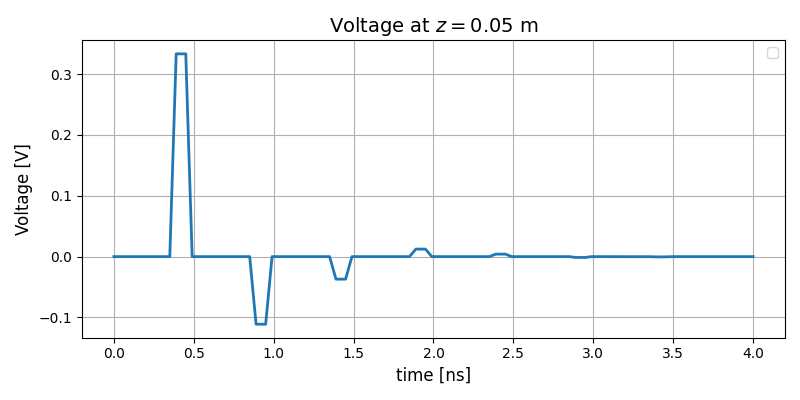
\includegraphics[scale=0.5]{figures/default.png}
    \caption{Bit behavior (voltage profile) under default settings}
    \label{fig:default}
\end{figure}

When $\tau_h$ becomes larger than 0.5 nanoseconds, interference between incident and reflected bits occur. The zero parts on the graph (in function of time) disappear and incidences and reflections influence each other, either positive or negative interference. This effect is shown in figure~\ref{fig:TH}.

\begin{figure}[h!]
    \centering
    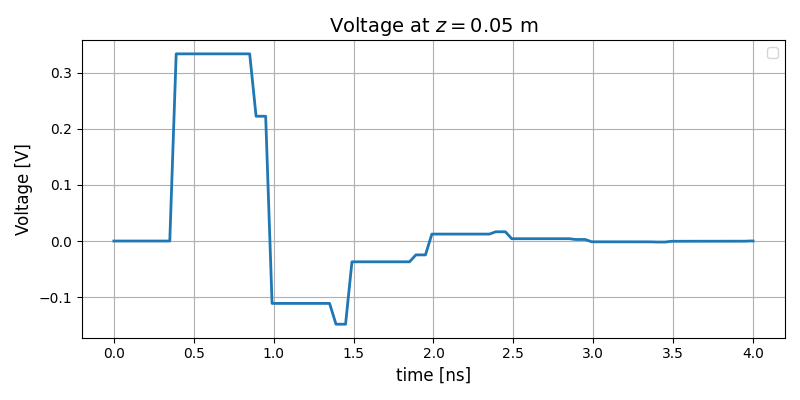
\includegraphics[scale=0.5]{figures/tau_h=0.5ns.png}
    \caption{$\tau_h = 500*10^{-12}$}
    \label{fig:TH}
\end{figure}

In the case of $\tau_h = \tau_r$, the bit has a triangular shape, as shown in figure~\ref{fig:sub1}. A curious effect can be noticed in the voltage profile when $\tau_r$ approaches 0. One would expect the bit to have square wave shape, but instead some non converging effects occur displayed in figure~\ref{fig:sub2}.

\begin{figure}[! h]
\centering
\begin{subfigure}{.5\textwidth}
  \centering
  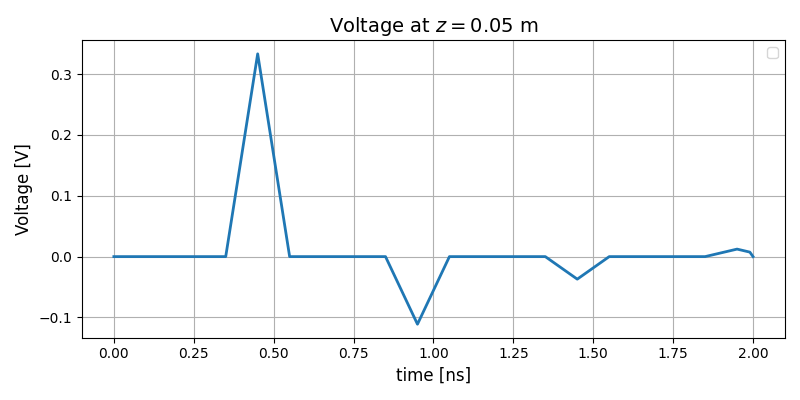
\includegraphics[width=.9\linewidth]{figures/tau_h_equals_tau_r.png}
  \caption{$\tau_h = \tau_r$}
  \label{fig:sub1}
\end{subfigure}%
\begin{subfigure}{.5\textwidth}
  \centering
  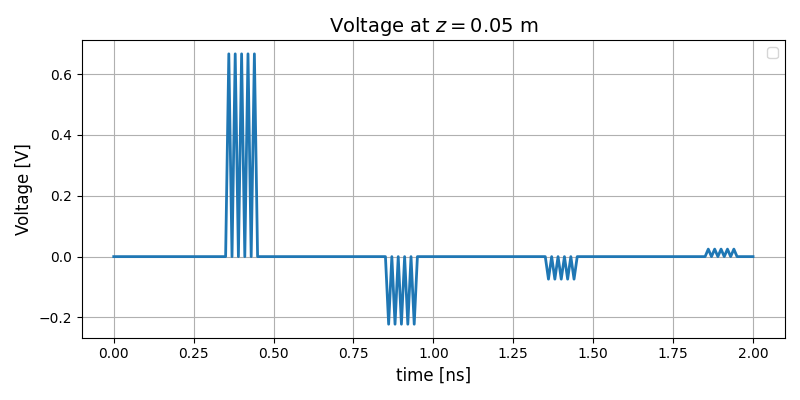
\includegraphics[width=.9\linewidth]{figures/tau_r naar 0.png}
  \caption{$\tau_r = 10^{-12}$}
  \label{fig:sub2}
\end{subfigure}
\caption{}
\label{fig:test}
\end{figure}

    \subsection{Effect of the Courant limit}

In function of the FDTD model, a discretization was performed of course, both in time and space. To justify the model physically, the steps in both time and space have to be chosen small enough. \\
The step in space $\Delta z$ has to be small enough to get rid of the wave phenomena. It cannot cross the boundary value of $\frac{\lambda_{min}}{10}$. The minimal wavelength $\lambda_{min}$ is simple to calculate as the fraction of the wave speed and the maximal frequency. The maximal frequency is given by the bandwith of the signal: $\frac{1}{\pi \tau_r}$. Considering the default settings ($\tau_r = 40.0e-12 s$ and $v = 200.0e6 m/s$) is the maximal step in space equal to $2.5133$ mm. Results with a bigger step in space can be ignored as they are physically incorrect.



The Courant limit is introduced to determine the maximal step in time. This limit states that $\Delta t$ can not be bigger than $\frac{\Delta z}{v}$. Just as in the case of $\Delta z$, results for $\Delta t$ bigger than this limit can be neglected since the time step $\Delta t$ will be bigger than the time it takes for the wave to cover a distance $\Delta z$ in that case. To illustrate this, the time step was brought up to $11e-12 s$ and the none converging graph is shown in figure~\ref{fig:test}.

\begin{figure}[! h]
\centering
\begin{subfigure}{.5\textwidth}
  \centering
  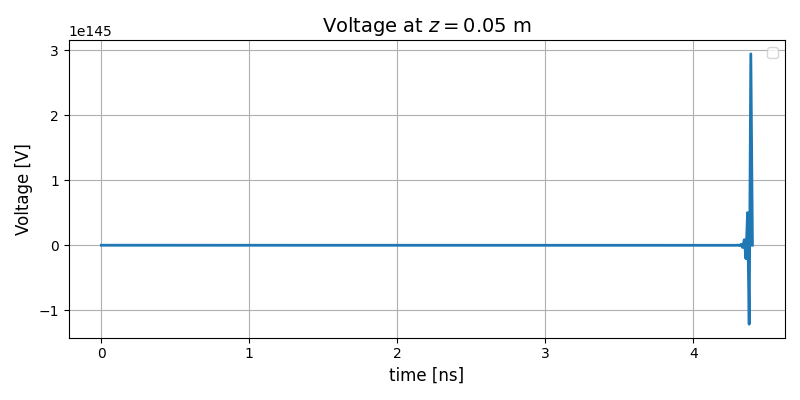
\includegraphics[width=.9\linewidth]{figures/alpha=1.1(z).png}
  \caption{Voltage for $\alpha = 1.1$ at $z = 0.05m$}
  \label{fig:dt1}
\end{subfigure}%
\begin{subfigure}{.5\textwidth}
  \centering
  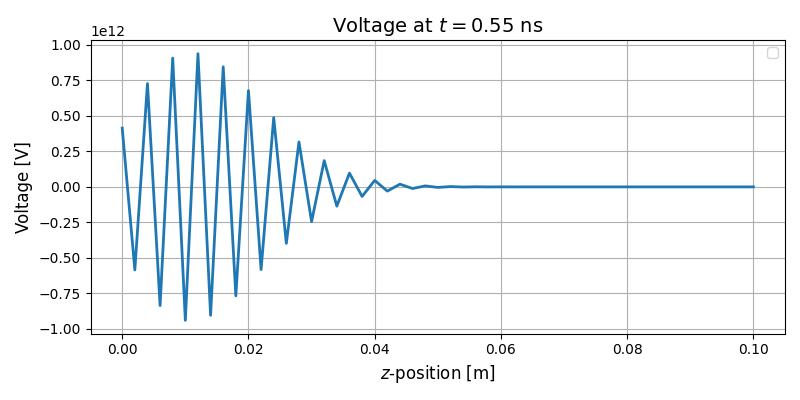
\includegraphics[width=.9\linewidth]{figures/alpha=1.1(t).png}
  \caption{Voltage for $\alpha = 1.1$ at $t = 0.55ns$}
  \label{fig:dt2}
\end{subfigure}
\caption{}
\label{fig:test}
\end{figure}

Applying the default values, $\Delta t$ exactly satisfies the Courant limit. This is the so called magic time step $(v\Delta z = \Delta t)$. When a time step smaller than the magic one is chosen, Gibbs phenomena occur.



The Courant factor $\alpha$, which also appears in the update equations, shows in what extend Gibbs phenomena are present. The maximal value of the Courant factor (to be physically relevant) is 1, which is also the perfect case. The lower the Courant factor becomes, the more Gibbs phenomena occur. This is illustrated in Figure~\ref{fig:alpha} for $\alpha$ being respectively 0.99 and 0.90. 

\begin{figure}[! h]
\centering
\begin{subfigure}{.5\textwidth}
  \centering
  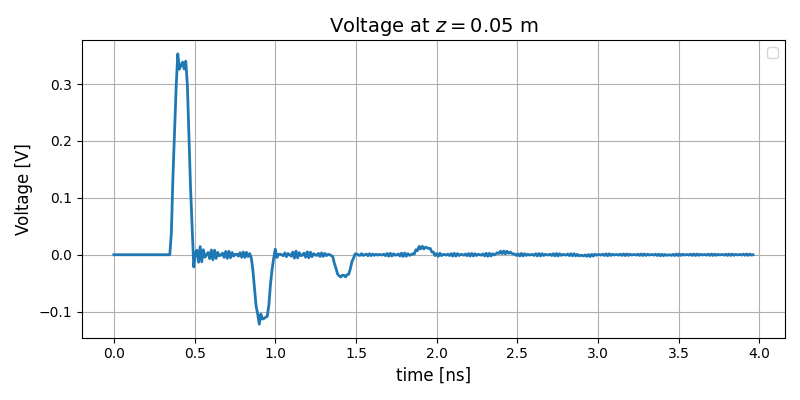
\includegraphics[width=.9\linewidth]{figures/alpha=0.99.png}
  \caption{$\alpha = 0.99$}
  \label{fig:dt1}
\end{subfigure}%
\begin{subfigure}{.5\textwidth}
  \centering
  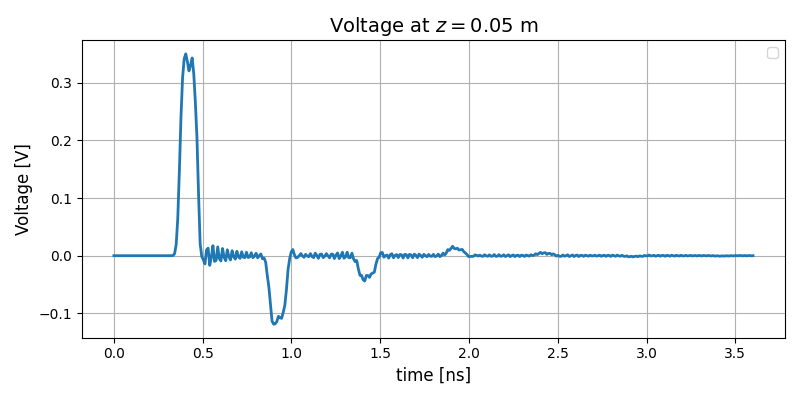
\includegraphics[width=.9\linewidth]{figures/alpha=0.90.png}
  \caption {$\alpha = 0.90$}
  \label{fig:dt2}
\end{subfigure}
\caption{}
\label{fig:alpha}
\end{figure}

    \subsection{Reflections and amplitude dampening}

In section (REF) the wave behavior of the voltage and current is discovered. To this end, the analysis of voltage waves at the boundaries for specific values of the generator resistance $R_g$ and load resistance $R_L$ is discussed. \\

Our first question concerns the entrance of the bit to the TL: the simulation starts at $t=0$ and the generator $\hat{e}_g$ produces a bit with amplitude $V_0$. Before the bit enters the TL, it meets the generator resistance $R_g$ and thus energy will be dissipated i.e. the voltage amplitude is dampened. This can be clarified by expressing Kirchoff's Voltage Law at the origin ($z=0$) of the TL;

\begin{align}
&\hat{e}_g(t) = (R_g + R_c)\hat{i}(0, t) \\
&\Rightarrow \hat{i}(0, t) = \frac{1}{R_g+R_c}\hat{e}_g(t)= \frac{1}{R_c}(\hat{v}^{+}(0, t) - \hat{v}^{-}(0, t)) \\
&\Rightarrow \hat{v}(0, t) = \hat{v}^{+}(0, t) =\kappa\hat{e}_g(0, t)\label{enter}.
\end{align}
The amplitude $V_0$ of the generated bit is reduced by a factor $\kappa = \frac{R_c}{R_g + R_c}$. Here, the role of the characteristic impedance becomes clear; at the beginning of the TL, the bit 'sees' it as input impedance, but does not dissipate energy to it; the bit amplitude remains constant during its passage through the TL. Indeed, the TL is lossless and only contains p.u.l capacitances and inductances (passive). One can observe two interesting cases:
\begin{itemize}
\item $R_g = 0 \Rightarrow \kappa = 1$\\ The generated bit freely enters the TL since it does not meet resistance.
\item $R_g = \infty \Rightarrow \kappa = 0$ \\ The circuit is open. The bit can not enter the TL.
\end{itemize}

Now, assume the bit is able to enter the transmission line ($R_g \neq \infty$) and propagates lossless towards the load with, obviously, constant speed $c$. Again, at the load ($z=d$), Kirchoff's Voltage Law must be satisfied. Consequently, a reflected wave with lower or equal amplitude will be originated (Figure \ref{fig:refl});
\begin{align}
&\hat{v}(d, t) = \hat{v}^{+}(d, t) + \hat{v}^{-}(d, t) = R_L\hat{i}(d, t) \\
&\Leftrightarrow \hat{v}^{+}(d, t) + \hat{v}^{-}(d, t) = \frac{R_L}{R_c}(\hat{v}^{+}(d, t) - \hat{v}^{-}(d, t)) \\
&\Leftrightarrow (1 + K_L)\hat{v}^{+}(d, t) = \frac{R_L}{R_c}(1 - K_L)\hat{v}^{+}(d, t) \\
&\Rightarrow K_L = \frac{R_L/R_c - 1}{R_L/R_c + 1} = \frac{R_L - R_c}{R_c + R_L}.
\end{align}


$K_L$ is also know as the reflection coefficient at the load. This constant determines how much of the amplitude is reflected back:
\begin{enumerate}
\item $R_L > R_c \Rightarrow K_L > 0$ \label{ref1} (Figure \ref{fig:damp} A) \\
	The voltage wave arriving at the load does not have enough power. Since the load impedance is not matched with the characteristic impedance, the voltage at the load must take the load impedance into account (KCL); the net voltage $\hat{v}$ is compensated such that its amplitude at the load is higher than the amplitude of the wave arriving at $R_L$; a backward wave is originated that satisfies $\hat{v}^{-} = K_L\hat{v}^{+}$, because than $$\hat{v}(d, t) = (1 + K_L)\hat{v}^{+}(d, t).$$ This might be counterintuitive, since one might think it violates the law of conservation of energy. Luckily, this is not true; comparing the input power to the power delivered to the load (first reflection) gives
	\begin{align}
		&P_{\text{in}} > P_L \\
		&\Leftrightarrow \frac{\kappa^2 V^2_0}{R_c} > \frac{(1 + K_L)^2\kappa^2V^2_0}{R_L} \\
		&\Leftrightarrow (R_L-R_c)^2 > 0 \label{Pw}.
	\end{align}
Equation (\ref{Pw}) is always true and the law of conservation of energy still holds. The reflected wave still contains $P_{\text{in}} - P_L$ power.
\item $R_L = R_c \Rightarrow K_L = 0$: MATCHING (Figure \ref{fig:damp} B)\\
	The energy of the forward wave is fully dissipated to the load. Maximum power is reached and there is no reflection back.
	
\item $R_L < R_c \Rightarrow K_L <0$ \\
	The same principle holds as in case \ref{ref1}, with the difference that the reflected wave amplitude has an opposite sign compared to the incident wave; that is, because the voltage wave arriving at the load contains too much energy.

\item $R_L \longrightarrow \infty \Rightarrow K_L \longrightarrow 1$ \\
	The electric circuit is open. When the voltage wave arrives at the end of the TL, it is fully reflected to the load and no energy is dissipated.
	
\end{enumerate}
Obviously, when the reflected wave arrives back at the generator it might be reflected back to the load, depending on the value of the generator impedance. In summary, the generated bit enters the TL weakened (\ref{enter}) and starts to move back and forth between the load impedance and generator impedance, whereby energy is dissipated and the amplitude reduces until the wave is fully dampened (REF VIDEO).

\begin{figure}[h!]
\centering
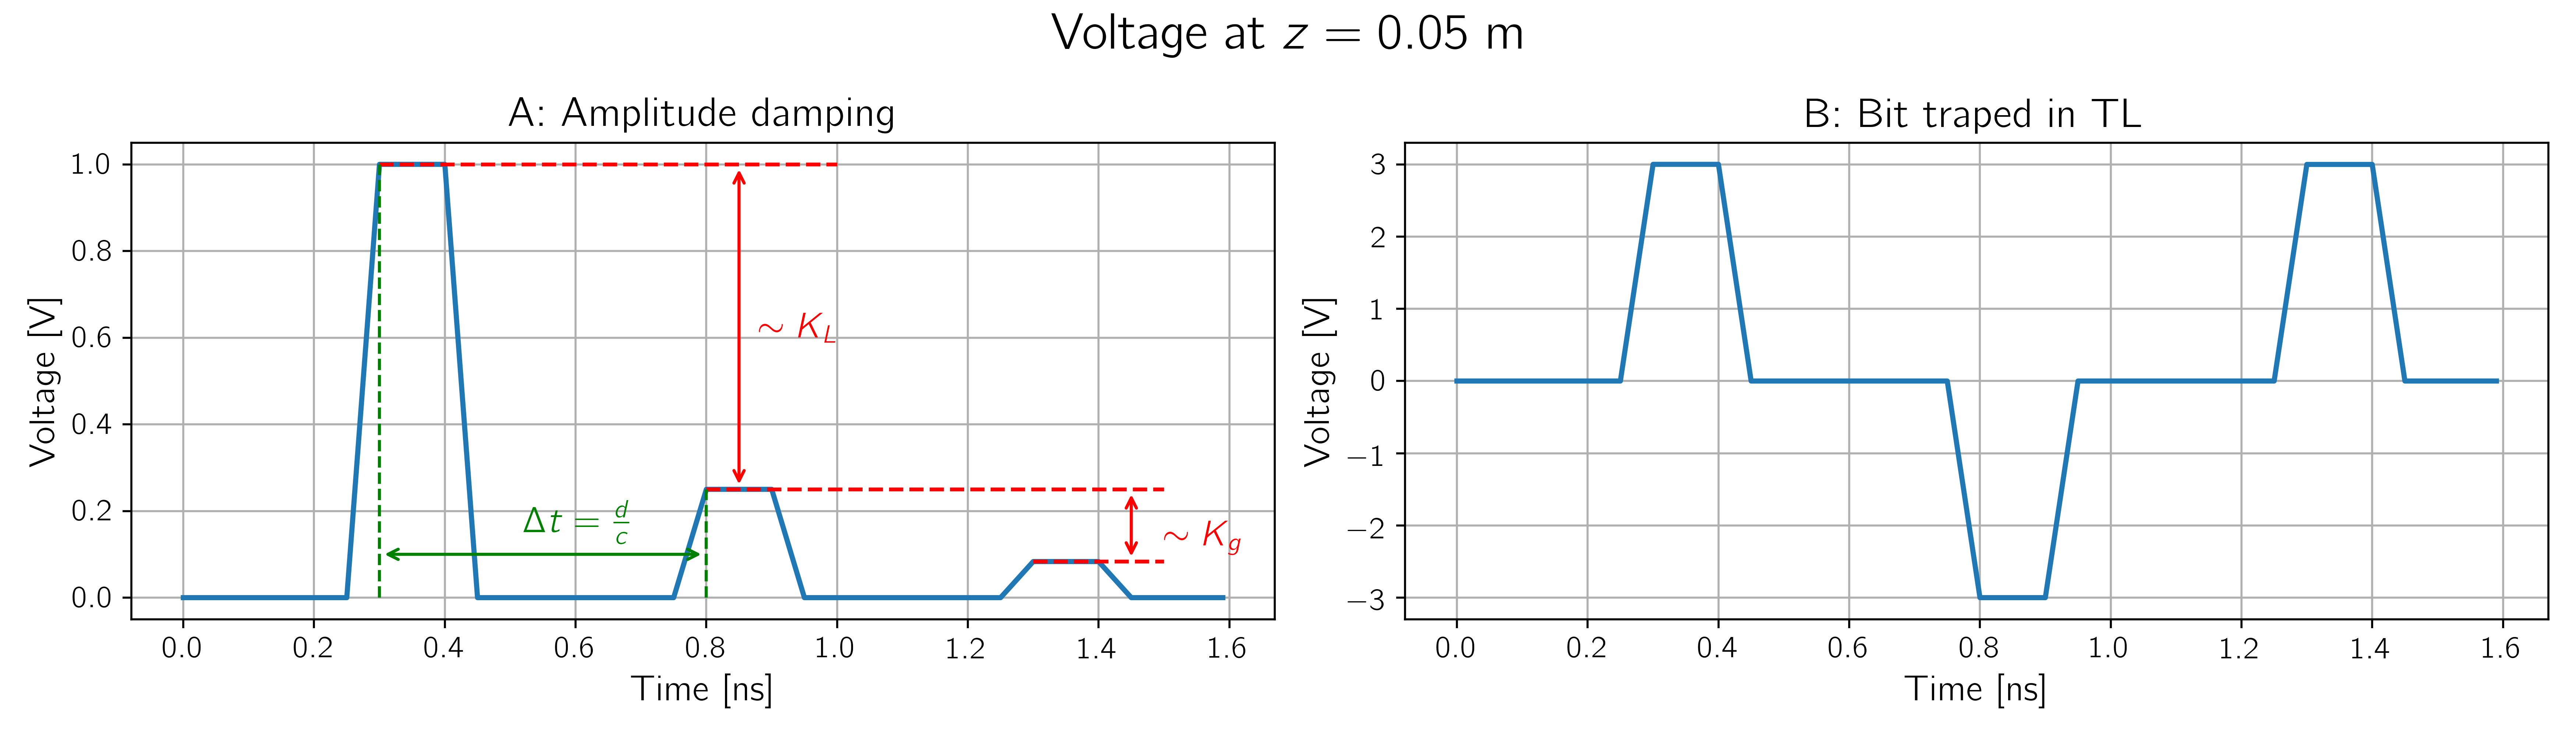
\includegraphics[width = \textwidth]{amplitudeplot.png}
\caption{FDTD simulations of a voltage wave traveling trough a TL. This wave moves with constant speed $c$ and is reflected at the load- and generator impedance with a damping factor $K_L$ resp. $K_g$. In A, the bit amplitude decreases as it meets an impedance. In B, the bit it trapped in the TL ($K_L\approx-1$ and $K_g \approx1$).}\label{fig:damp}
\end{figure}

\begin{figure}[h!]
\centering
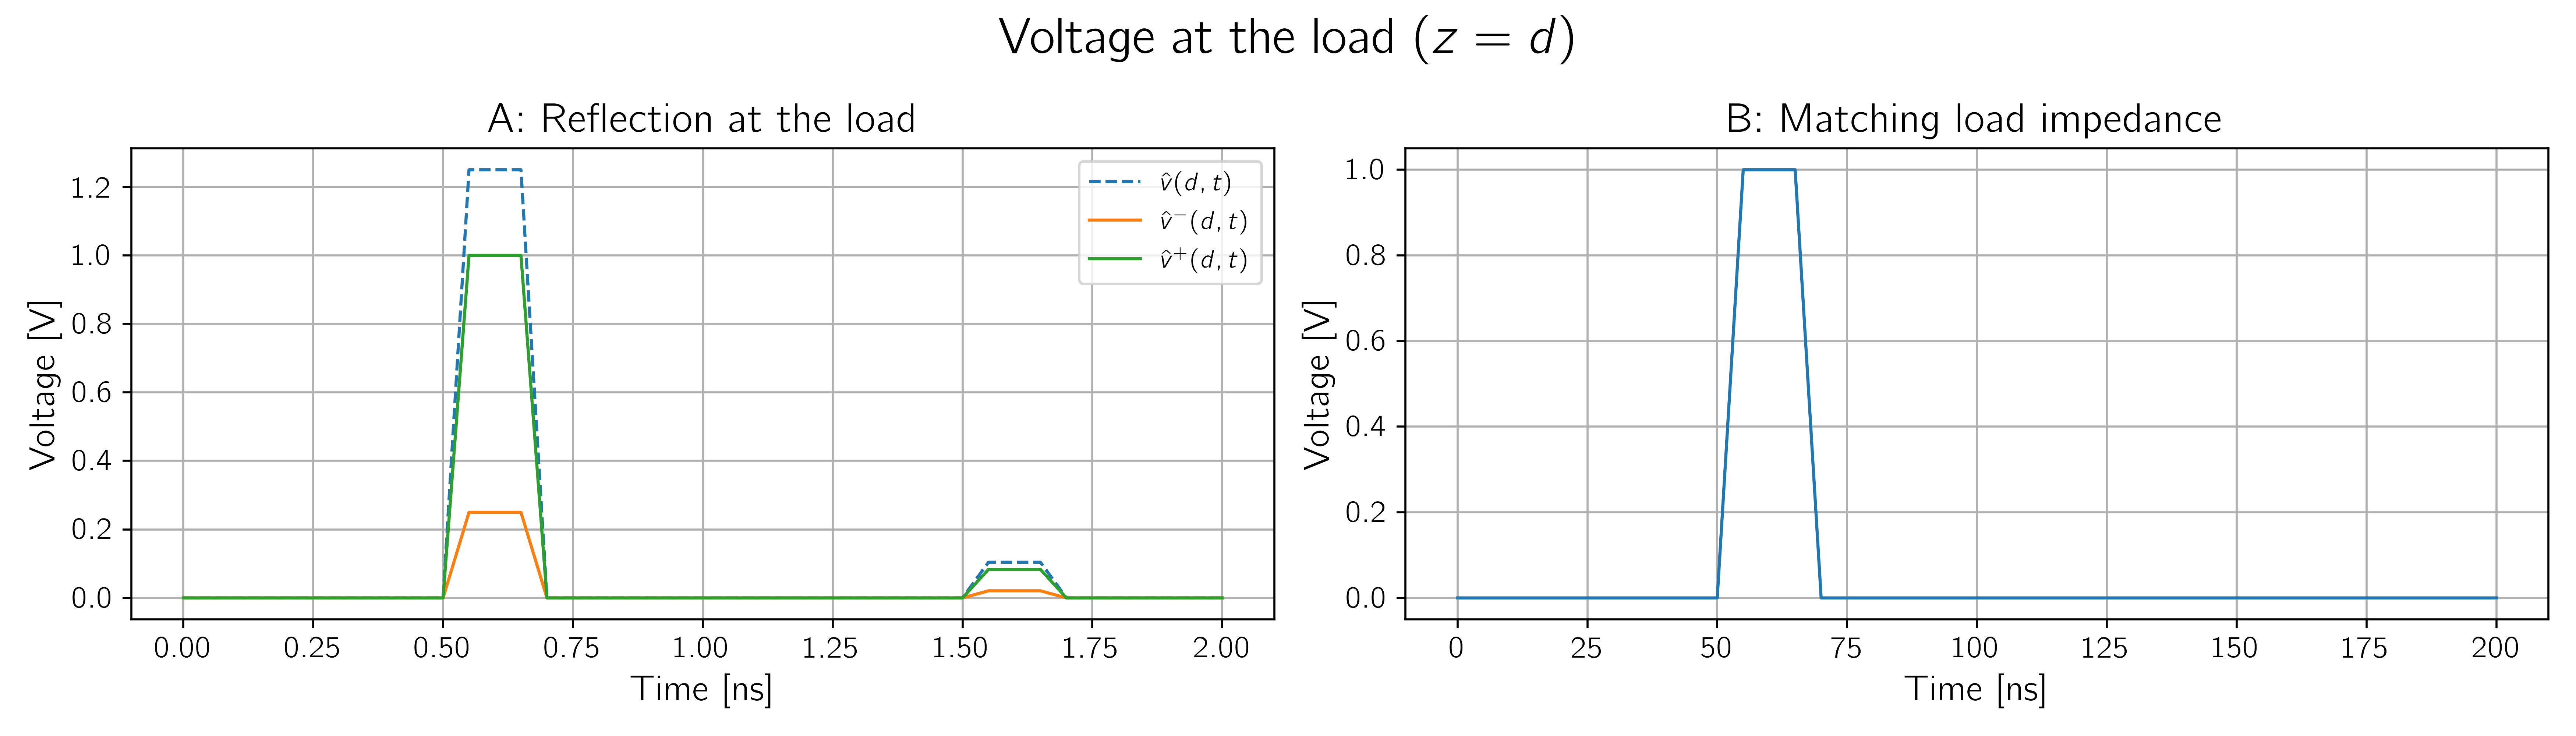
\includegraphics[width = \textwidth]{reflection.png}
\caption{Plot of voltage wave (FDTD simulation) at the load and decomposed into its forward $\hat{v}^{+}$ and backward $\hat{v}^{-}$ component.}\label{fig:refl}
\end{figure}

    \subsection{Resistive and Capacitive load}

\subsubsection{Adjusted boundary conditions}

Adding a capacitance in parallel with the load as depicted in figure \ref{fig:Rl_Cl} gives rise to some adjustements to the voltage update function at $z=0$.

\begin{figure}
    \centering
    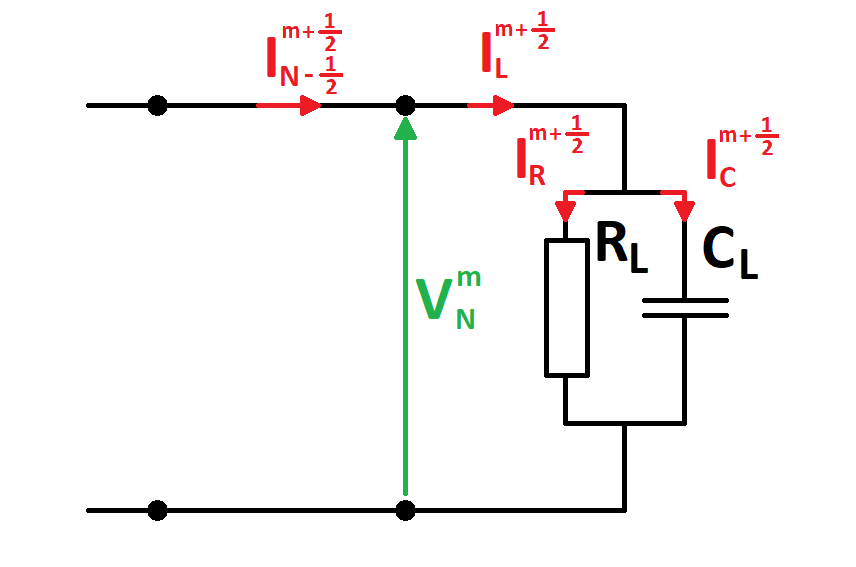
\includegraphics[scale=0.35]{BC2_cap}
    \caption{Load with capacitance}
    \label{fig:Rl_Cl}
\end{figure}

Kirchoff's current law states now that
\begin{equation}
    I^{m+\frac{1}{2}}_{L} = I^{m+\frac{1}{2}}_{R} + I^{m+\frac{1}{2}}_{C}.
    \label{IL2}
\end{equation}
Using Kirchoff's voltage law at the resistor gives
\begin{align}
    I^{m+\frac{1}{2}}_{R} & = \frac{V^{m+\frac{1}{2}}_{N}}{R_{L}}\nonumber\\
    & = \frac{V^{m}_{N}+V^{m+1}_{N}}{2R_{L}}
    \label{IR}
\end{align}
The relation between the current and the voltage at the capitor is given by
\begin{equation}
    \hat{i} = C\frac{\partial \hat{v}}{\partial t}.
\end{equation}
For a first order FDM this turns into
\begin{equation}
    I^{m+\frac{1}{2}}_{C} = C_{L}\frac{V^{m+1}_{N} - V^{m}_{N}}{\Delta t}.
    \label{IC}
\end{equation}
Substituting (\ref{IR}) and (\ref{IC}) into (\ref{IL2}) gives
\begin{equation}
    I^{m+\frac{1}{2}}_{L} = \left(\frac{1}{2R_{L}}+\frac{C_{L}}{\Delta t}\right)V^{m+1}_N + \left(\frac{1}{2R_{L}}-\frac{C_{L}}{\Delta t}\right)V^{m}_N
\end{equation}
and can be rewritten as
\begin{equation}
    \tilde{I}^{m+\frac{1}{2}}_{L} = \frac{R_{c}}{2Z_{2}}V^{m+1}_N + \frac{R_{c}}{2Z_{1}}V^{m}_N
    \label{IL2_final}
\end{equation}
with
\begin{align}
    Z_{1} &= \left(\frac{1}{R_{L}}-2\frac{C_{L}}{\Delta t}\right)^{-1} = \frac{R_{L}\Delta t}{\Delta t - 2 C_{L}R_{L}} \nonumber\\
    Z_{2} &= \left(\frac{1}{R_{L}}+2\frac{C_{L}}{\Delta t}\right)^{-1} = \frac{R_{L}\Delta t}{\Delta t + 2 C_{L}R_{L}} \label{eq:Z}
\end{align}
Substituting (\ref{IL2_final}) into the adjusted voltage update function at $z=d$ yields
\begin{equation}
    V^{m+1}_{N} = K'_{2}V^{m}_N + 2\kappa'_{2}\tilde{I}^{m+\frac{1}{2}}_{N-\frac{1}{2}},
\end{equation}
where
\begin{align}
    K'_{2} & = \frac{Z_{2}}{Z_{1}}\frac{Z_{1}-\alpha R_{c}}{Z_{2}+\alpha R_{c}},\\
    \kappa'_{2} & = \frac{\alpha Z_{2}}{Z_{2}+\alpha R_{c}}.
\end{align}
are the new dimensionless constants.

\subsubsection{Influence of C}

First thing to notice is that when $C_{L} = 0$ then $K'_{2} = K_{2}$ and $\kappa'_{2} = \kappa_{2}$. This is a good
sign since it stays consistent with the previous update equation.\\
Secondly in relations \ref{eq:Z} there is a time step dependecy, hence the two dimensionless
coefficients in the boundary update function at $z=d$ are also dependent on the implemented time step. Let's consider a
well chosen time step and just look at the effect of changing $C_{L}$.
\begin{itemize}
    \item $C_{L} \rightarrow 0$ :
        $K'_{2} \rightarrow K_{2}$ and $\kappa'_{2} \rightarrow \kappa_{2}$, initial situation
    \item $C_{L} \rightarrow \infty$ :
        $ K'_{2} \rightarrow 1$ and $\kappa'_{2} \rightarrow 0$, fully reflected wave
    \item $C_{L} \rightarrow \frac{\Delta t}{2R_{L}}$ :
        $K'_{2} \rightarrow \frac{Z_{2}}{Z_{2}+\alpha R_{C}}$ and $\kappa'_{2} \rightarrow \frac{2\alpha Z_{2}}{Z_{2}+\alpha R_{C}}$, this shows that the division by zero for $Z_1$ does not lead to any problems.
\end{itemize}

\begin{figure}[H]
    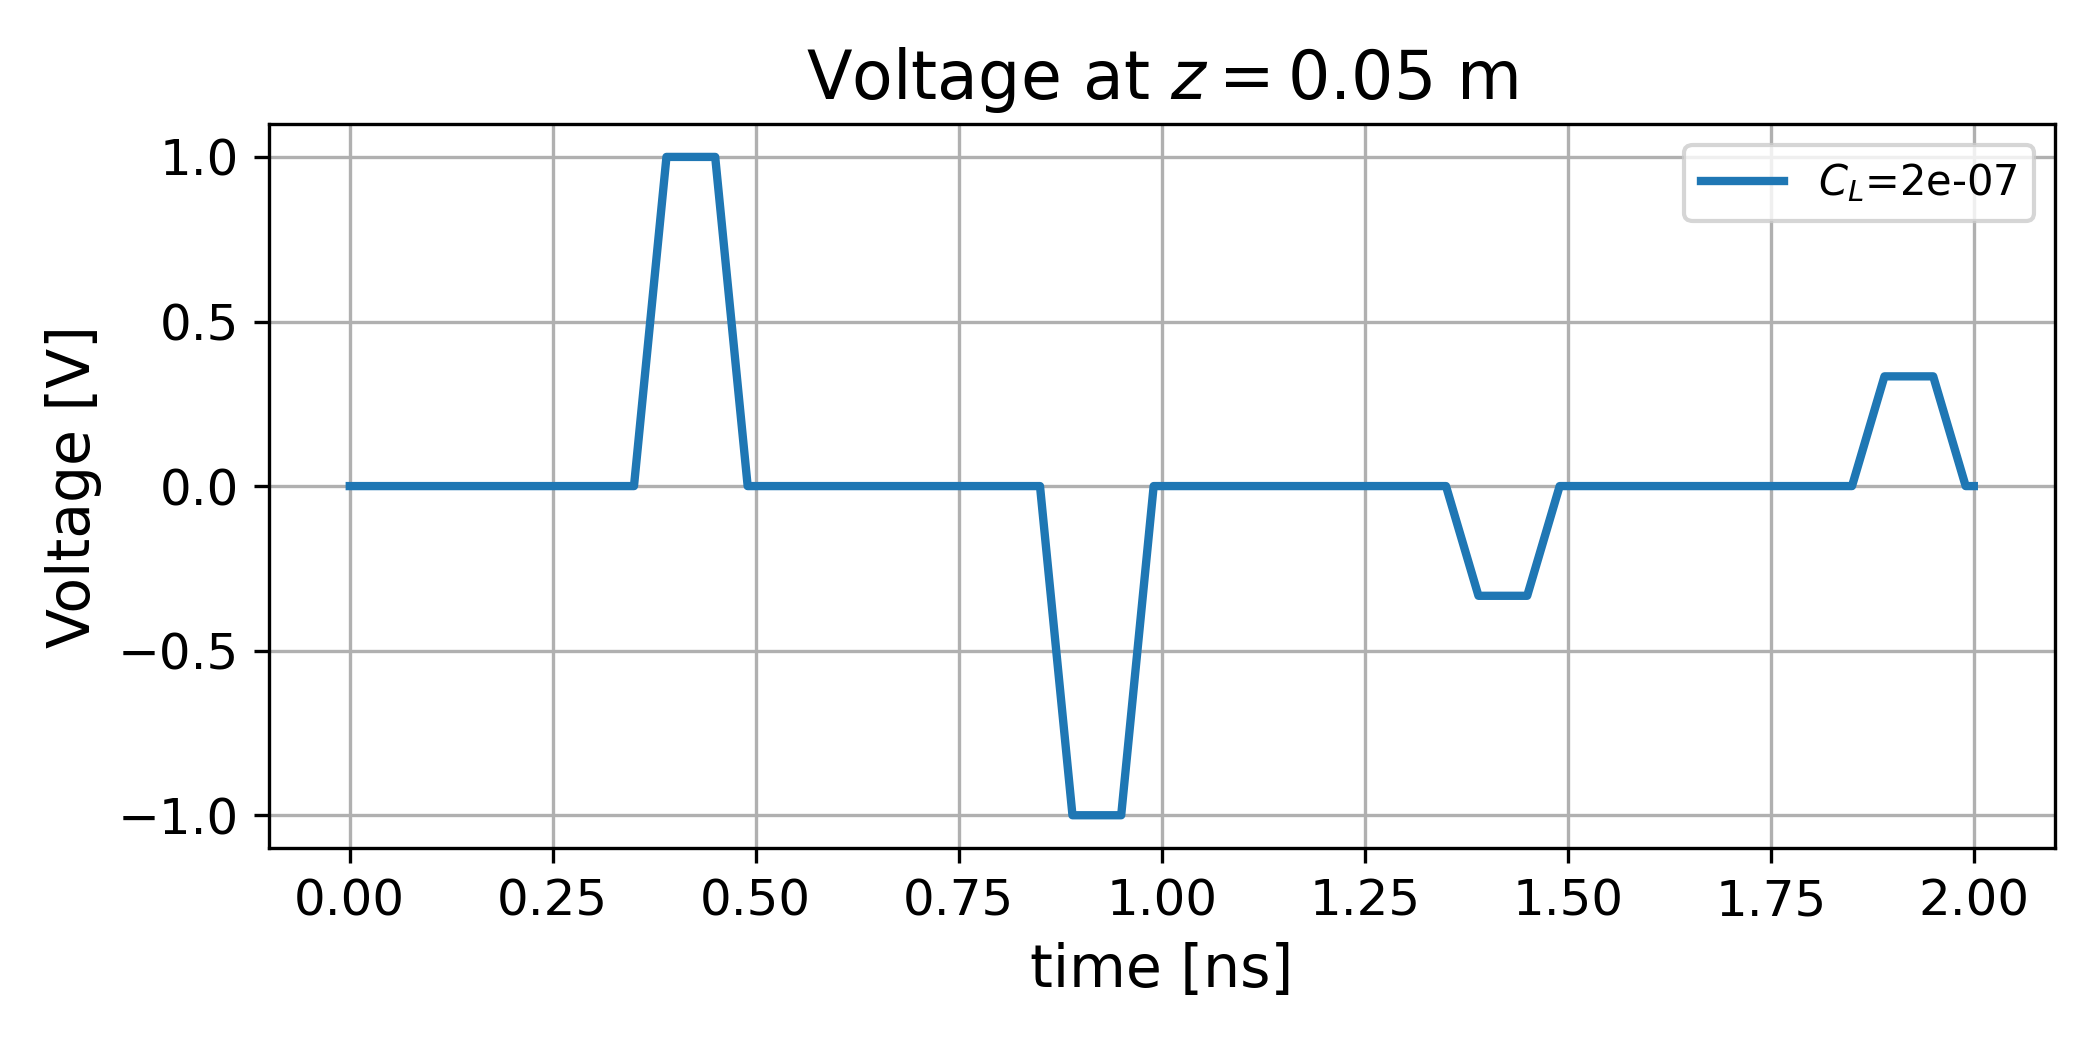
\includegraphics[scale=0.5]{example_C=2e-07_time.png}
    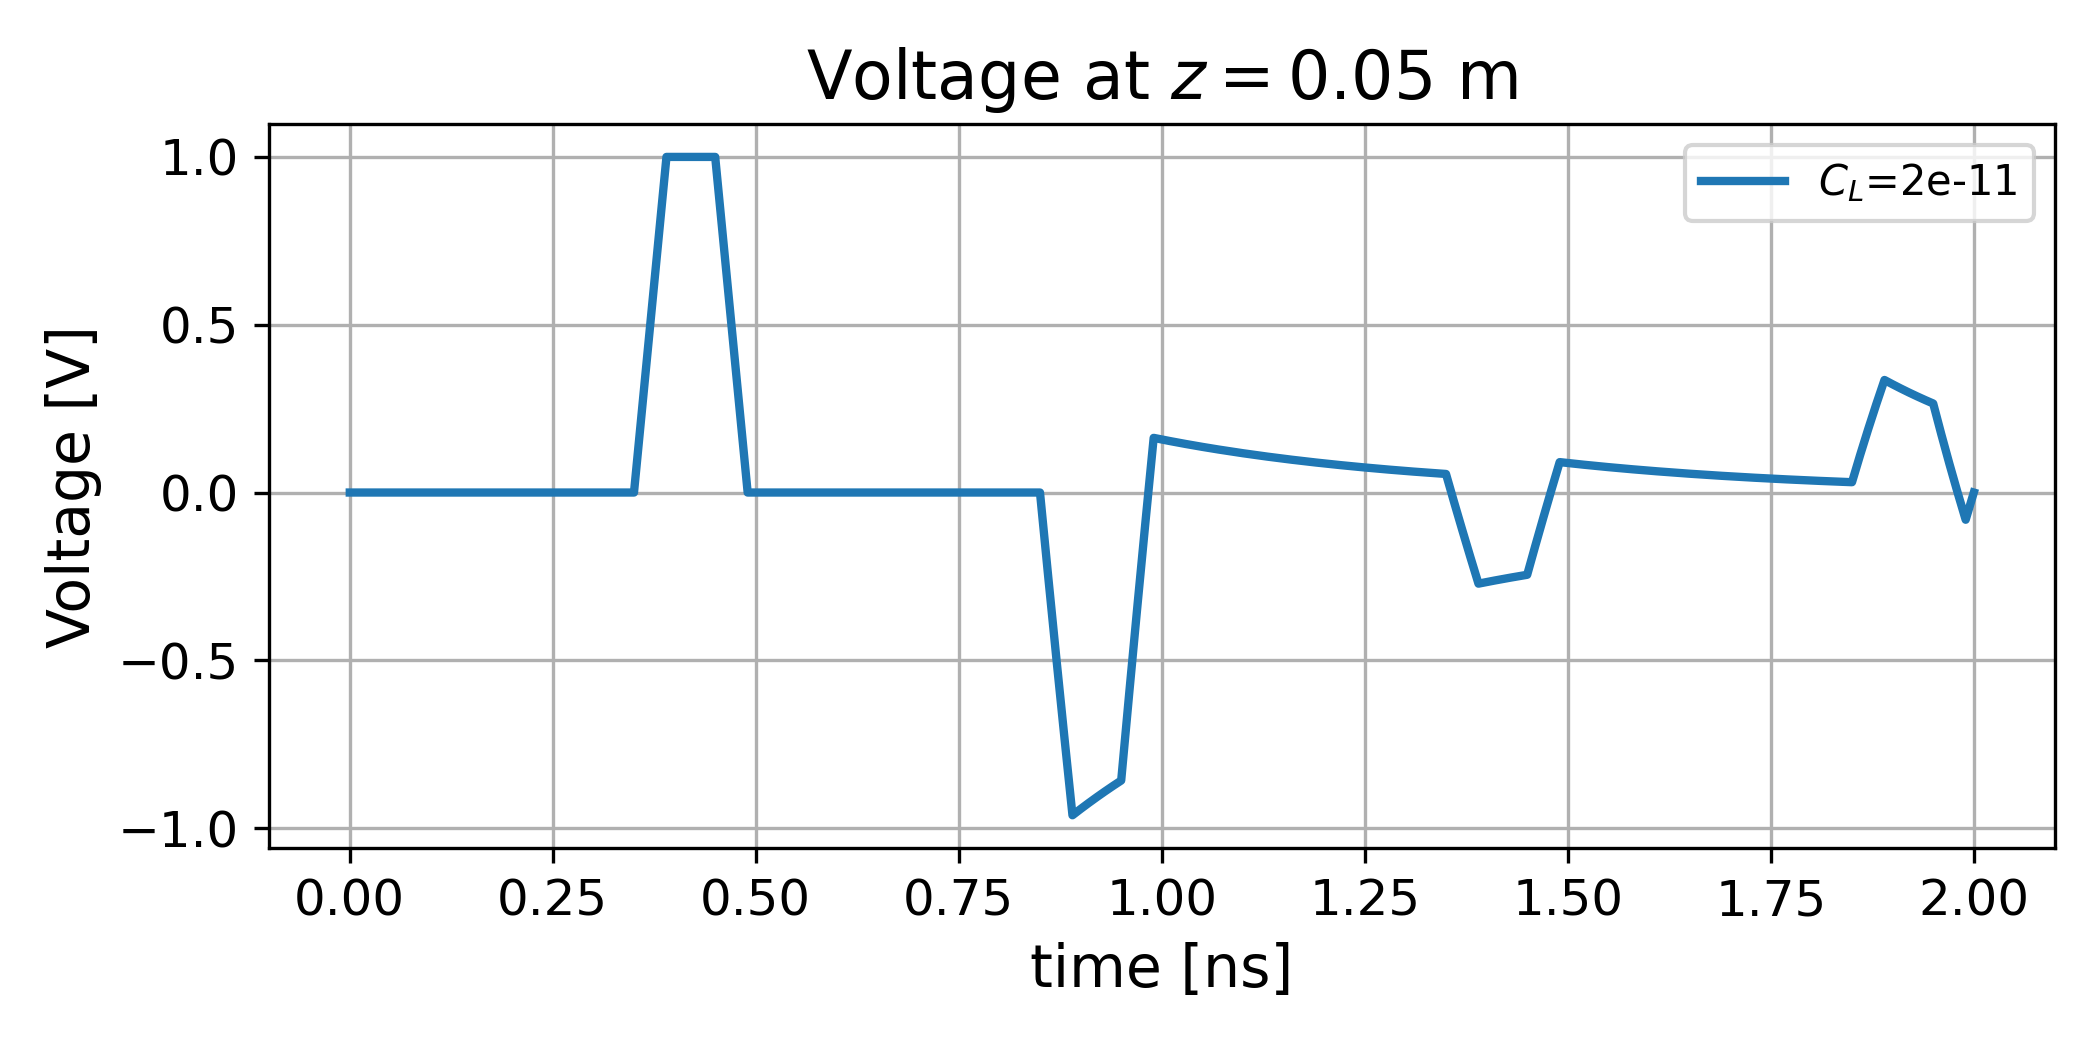
\includegraphics[scale=0.16]{example_C=2e-11_time.png}

    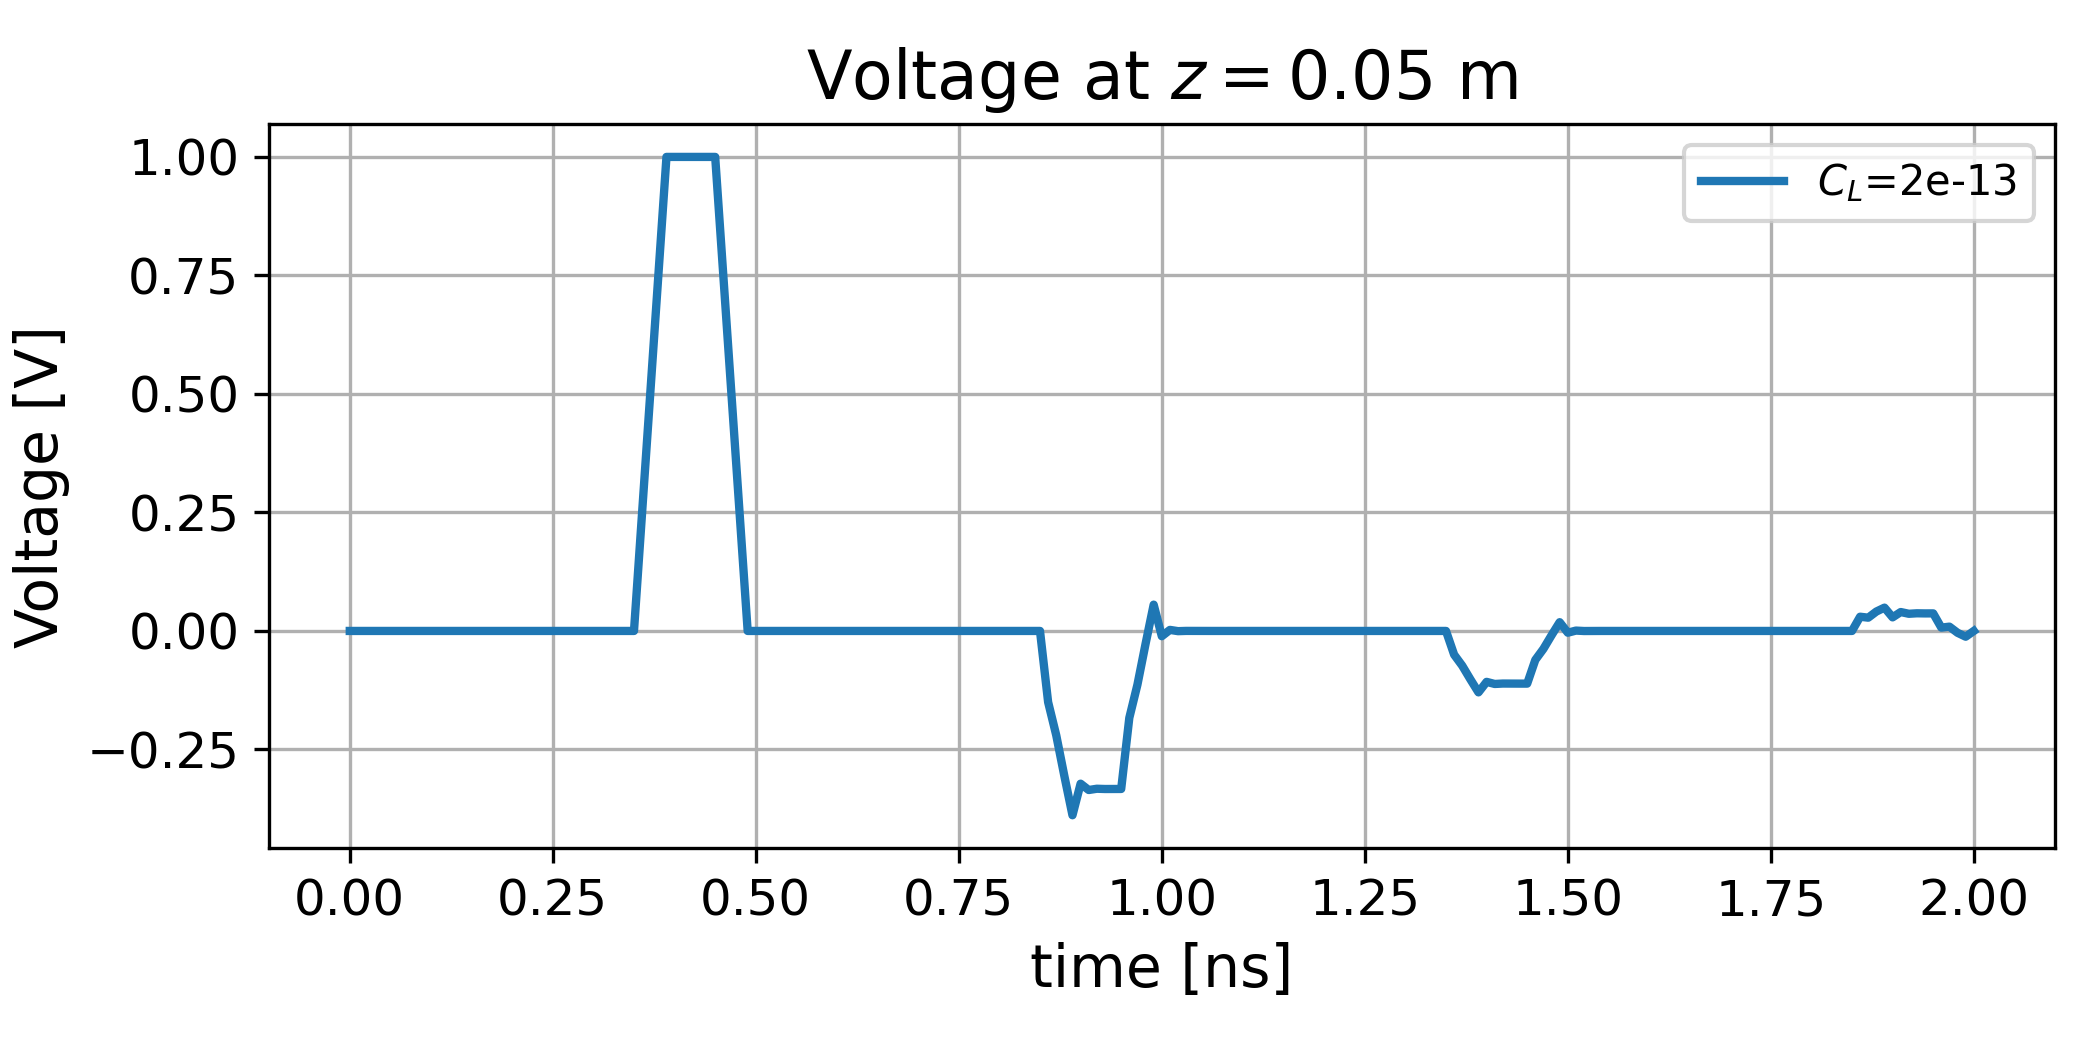
\includegraphics[scale=0.5]{example_C=2e-13_time.png}
    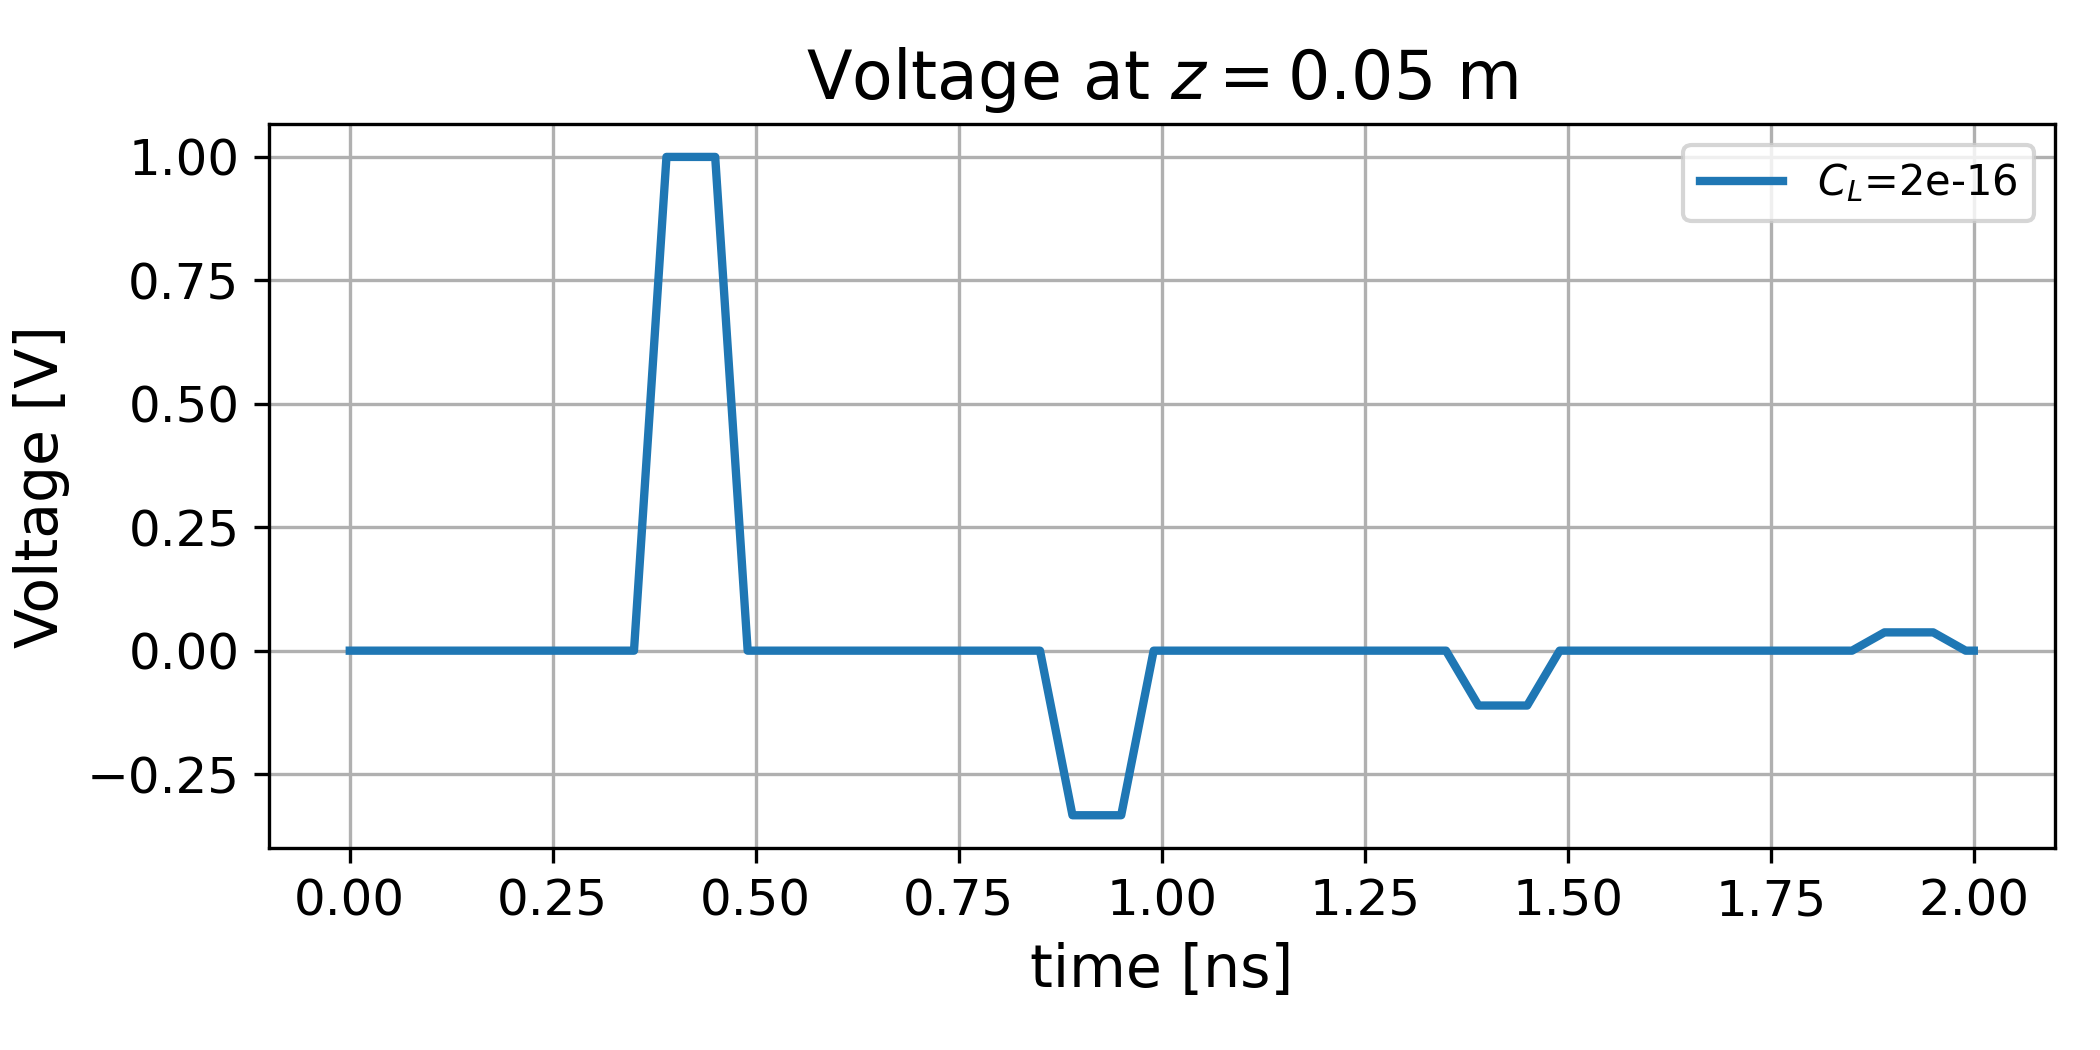
\includegraphics[scale=0.5]{example_C=2e-16_time.png}
    \caption{Different values for the load capacitance}
    \label{fig:effect_CL}
\end{figure}

From figure \ref*{fig:effect_CL} the following obesrvations can be made:
\begin{itemize}
    \item For large values of the capacitance no energy loss will occur at the load, i.e. the amplitude of the voltage does not change when passing the load. The capacitor has enough capacitance to store the whole bit and return it to the transmision line.
    \item For intermediate values for the capacitance, i.e. $C_L = 2e-11$, the decharging of the capacitor can clearly be seen (exponetial drop).
    \item When the capacitance gets very low its effect gets negligible.
\end{itemize}

\section{Biomedical application}

Since this report was written by three students in biomedical engineering, this section looks shortly in the application of transmission line theory in this field of engineering. A small study of literature was conducted to gather some insight in this topic.
When one thinks of electric signals related to the human body, of course the nervous system immediately comes to mind. Neuro-engineering is a very active field within biomedical engineering. The foundation of modelling nerve impulses was built by Hodgkin and Huxley in 1951. They constructed a model to replicate the specific way






\end{document}
